%% LyX 2.3.6 created this file.  For more info, see http://www.lyx.org/.
%% Do not edit unless you really know what you are doing.
\documentclass[english,11pt,3p,number,sort&compress]{elsarticle}
\usepackage[T1]{fontenc}
\usepackage[latin9]{inputenc}
\usepackage{geometry}
\geometry{verbose,tmargin=2cm,bmargin=2cm,lmargin=2cm,rmargin=2cm,headheight=2cm,headsep=2cm,footskip=1cm}

\usepackage{color}
\usepackage{array}
\usepackage{float}
\usepackage{algorithm2e}
\usepackage{amsmath}
\usepackage{amssymb}
\usepackage{stmaryrd}
\usepackage{bm}
\usepackage{graphicx}
\usepackage{lipsum} 

%%%%%%%%%%%%%%%%%%%%%%%%%%%%%% LyX specific LaTeX commands.
%% Because html converters don't know tabularnewline
\providecommand{\tabularnewline}{\\}

%%%%%%%%%%%%%%%%%%%%%%%%%%%%%% User specified LaTeX commands.
%\usepackage[latin1]{inputenc}

\usepackage{natbib}
\usepackage{dsfont}
\usepackage{comment}
\usepackage{ifthen}    
\usepackage{lscape}
\usepackage{graphicx}
\usepackage{hyperref}

\usepackage[subpreambles=true]{standalone}
\usepackage{xspace}
\usepackage[percent]{overpic}

%tikz stuff
\usepackage[customcolors]{hf-tikz}
\usepackage{tikz}
\usepackage{pgfplots}
\usetikzlibrary{calc,shadings,patterns,tikzmark, plotmarks, spy, 
pgfplots.polar, external, matrix, shapes.symbols,shadings,shapes, 
decorations.shapes,decorations.pathmorphing,fit,backgrounds}
\pgfplotsset{compat=1.10}   %% <-- this added

\usepgfplotslibrary{groupplots}
\usetikzlibrary{calc}
\usepackage{pgfplotstable}

\usepackage{xcolor}

% WARNING: This folder must exist
\tikzexternalize[prefix=./figs_pgfplots/tikz/]

\newcommand{\includetikz}[1]{%
	\tikzsetnextfilename{#1}%
	\input{#1}%
}

% compatibility for pgf figure
\pgfplotsset{compat=newest}

\hypersetup{urlcolor=blue, colorlinks=true}

% Useful when sending to journals.
% Do not provide path to figures in includegraphics comand. Set them
% here instead.
\graphicspath{ {./figs/} }

% path to tikz files. Do not use path in \includetikz command
\makeatletter
\def\input@path{{./figs_pgfplots/}{./fig/}}
\makeatother

\makeatletter
\@ifundefined{showcaptionsetup}{}{%
 \PassOptionsToPackage{caption=false}{subfig}}
\usepackage{subfig}
\makeatother

\usepackage{babel}

\newcommand{\giovane}{\color{red}{\bf\Large GA} \color{cyan} }

\journal{Engineering with Computers}

\begin{document}

\begin{frontmatter}{}

%Um primeiro título
\title{A primal double-hybrid finite element method to solve tridimensional compressible, quasi-incompressible and incompressible elasticity using de Rham compatible H(div)-L2 spaces}

\author[uni]{Giovane Avancini}

\ead{giovanea@unicamp.br}

\author[uni]{Nathan Shauer}

\ead{shauer@unicamp.br}

\author[uni]{Hugo Luiz Oliveira}

\ead{hluiz@unicamp.br}

\author[uni]{Philippe R. B. Devloo}

\ead{phil@unicamp.br}

\address[uni]{Universidade Estadual de Campinas, R. Josiah Willard Gibbs 85 - Cidade Universitaria, Campinas SP, Brazil, CEP 13083-839}

%Definir se vamosar usar double-hybrid ou hybrid-hybrid. Adotei a segunda opção por enquanto
\begin{abstract}
	This work is devoted to the development of a novel primal double-hybrid finite element formulation for the solution of tridimensional compressible, quasi-incompressible and incompressible elasticity problems. Hybrid-mixed methods are typically derived from an extended variational principle, where the requirement for the interlement continuity of the functions spaces is relaxed and weakly imposed using Lagrange multipliers over the element interfaces. In this sense, we propose the usage of a De Rham compatible pair H(div)-L2 for displacements and pressure, respectively. H(div) spaces naturally guarantees the continuity of the normal displacement across elements, so the tangential component conformity can be retrieved at the expense of introducing a shear stress approximation on the element edges. This leads to a semi-hybrid approach with two Lagrange multipliers so solving a saddle-point problem is inevitably even in the compreesible regime. To overcome this drawback, the shear stress can be further hybridized a second time and statically condensed to recover a positive-definite block matrix that depends on the primal variable components. In fact, there is still the need of solving a saddle point system when the bulk modulus tends to infinity, however, results have shown that this approach presents a superior stability compared to the semi-hybrid formulation. The stability, consistency and local conservation features are discussed in details. The formulation is tested and verified using 3D benchmarks for which analytical and/or numerical solutions are available, exhibiting optimal convergence rate independent of the poisson coefficient. The proposed methodology is also applied to a real-world problem, where the performance of the method is assessed in terms of accuracy and computational cost.
\end{abstract}
\begin{keyword}
\textit{Hybrid finite elements; Elasticity; H(div) approximation space; Incompressibility; Local conservation}
\end{keyword}

\end{frontmatter}{}

\section{Introduction}

{\giovane A first shot, please give your contributions}
In the context of linear elasticity, several numerical methods have been developed in the past years. The most used one is the Finite Element Method (FEM). Using a continuous Galerkin approach to approximate the displacements may lead to shear-locking phenomenon due to spurious energy modes under bending \cite{bletzinger2000unified,belytschko1985stress} or volume-locking under quasi or full incompressibility, as the stresses go to infinity \cite{neto2005f,cervera2003mixed}.

There are different ways in the literature to overcome these drawbacks. One possible choice is to employ a mixed formulation \cite{brezzi2012mixed,arnold1988new} where the displacements and the stresses (or pressure) are approximated independently - i.e. the Taylor Hood elements \cite{taylor1973numerical} fulfill the \textit{inf-sup} condition yielding stable results for incompressible regime. This kind of approximation, on the other hand, is not locally conservative as it does not satisfy the divergence constraint in a strong manner. Another possibility is to use hybrid methods where the interelement continuity of a given field is broken and weakly imposed by means of a Lagrange multiplier (see for instance \cite{raviart1977primal,harder2016hybrid,farhloul1997dual}).

In this work we extend the semi-hybrid approach proposed in \cite{carvalho2024semi} for Stokes flows to elasticity problems, developing a new formulation by performing a second hybridization on the tangential stresses. This formulation is based on a de Rham compatible pair $H(\text{div})-L^2$ for displacements and pressure. The $H(\text{div})$ functions are constructed using a systematic methodology described in \cite{devloo2022efficient,de2013new}.


\section{Preliminaries and notation}
{\giovane should we make a section for this?}

\section{Elasticity problem \label{sec:Governing-equations}}

In this section, the governing equations for the linear elasticity problem shall be defined. Firstly, the primal displacement based formulation is presented, followed by the mixed version introducing the pressure as an indepent variable.

\subsection{Strong form}

Let $\Omega \in \mathbb{R}^d : d\in\{2,3\}$ be an open domain with Lipschitz boundary $\partial\Omega=\partial\Omega_D\cup\partial\Omega_N$, where $\partial\Omega_D$ and $\partial\Omega_N$ stand for the boundary portion where Dirichlet and Neumann boundary conditions are applied, respectively. The conservation of linear momentum for a generic continuum body is given by::
\vskip-.2cm
\begin{equation} \label{eq:momentum}
		-\nabla \cdot \boldsymbol{\sigma} - \mathbf{b} = \mathbf{0} \hspace{0.2cm} \text{in } \Omega \text{,}
\end{equation}

\noindent where $\mathbf{b} \in L^2(\Omega)$ is the body forces vector and $\boldsymbol{\sigma} \in H(\text{div},\Omega)$ denotes the Cauchy stress tensor.

The Generalized Hook law relates the stresses and strains in a isotropic body as:
\vskip-.2cm
\begin{equation} \label{eq:hook}
    \boldsymbol{\sigma} = 2\mu \boldsymbol{\varepsilon} + \lambda \text{tr}(\boldsymbol{\varepsilon}) \mathbf{I}^d \text{,}
\end{equation}

\noindent where $\mathbf{I}^d$ is the identity matrix of dimension $d$, $\mu$ and $\lambda$ are known as Lam\'{e} constants, given respectively by
\vskip-.2cm
\begin{equation}
	\lambda = \frac{E\nu}{(1+\nu)(1-2\nu)} \text{,} \quad \mu = \frac{E}{2(1+\nu)} \text{,}
\end{equation}

\noindent with $E$ and $\nu$ standing for the Young modulus and Poisson coefficient. The infinitesimal strain tensor $\boldsymbol{\varepsilon}$ is the symmetric countepart of the displacement gradient:
\vskip-.2cm
\begin{equation} \label{eq:strain}
    \boldsymbol{\varepsilon}=\frac{1}{2}(\nabla\mathbf{u}^T+\nabla\mathbf{u}) \text{.}
\end{equation}

By substituting Eqs. \eqref{eq:hook} and \eqref{eq:strain} into Eq. \eqref{eq:momentum}, the pure displacement boundary value problem, also known as the Navier-Cauchy problem, reads: find displacement $\mathbf{u} \in H^2_D(\Omega)$, where $H^2_D(\Omega)=\{\mathbf{u}\in H^2(\Omega) : \mathbf{u}\lvert_{\partial\Omega_D} = \mathbf{u}_D  \}$, such that
\vskip-.2cm
\begin{equation} \label{eq:navier-cauchy}
	\begin{aligned}
		-\mu\nabla^2\mathbf{u} -\left(\mu+\lambda \right)\nabla\left(\nabla \cdot \mathbf{u} \right) - \mathbf{b} = \mathbf{0} \hspace{0.2cm} \text{in } \Omega \text{,}&\\
		\mathbf{u} = \mathbf{u}_D \hspace{0.2cm} \text{on } \partial\Omega_D \text{,}&\\
		\boldsymbol{\sigma} \cdot \mathbf{n} = \mathbf{t} \hspace{0.2cm} \text{on } \partial\Omega_N \text{,}&
	\end{aligned}
\end{equation}

\noindent where {\giovane check the following spaces} $\mathbf{u}_D \in H^{1/2}(\partial\Omega_D)$ and $\mathbf{t} \in H^{-1/2}(\partial\Omega_N)$ are the prescribed displacements and tractions on $\partial\Omega_D$ and $\partial\Omega_N$, respectively.

The elasticity problem can also be formulated using two state variables by applying the additive decomposition on the Cauchy stress tensor in its deviatoric and hydrostatic counterparts, resulting in:
\vskip-.2cm
\begin{equation} \label{eq:stress-decomposition}
	\boldsymbol{\sigma} = \boldsymbol{\sigma}' - p\mathbf{I}^d \text{,}
\end{equation}

\noindent where p is the hydrostatic pressure, computed as
\vskip-.2cm
\begin{equation} \label{eq:pressure}
	p = -\kappa \text{tr}(\boldsymbol{\varepsilon}) \text{,}
\end{equation}

\noindent with $\kappa$ standing for the bulk modulus, which for the generalized tridimensional case, comes from the expression $\kappa=\frac{2\mu+3\lambda}{3}$. Its value for the plane stress and plane strain hypothesis can also be derived by imposing the constraints on each case {\giovane should we put the derivation of the bulk modulus for the plane analyses in an appendix?}. Plugging Eqs. \eqref{eq:pressure} and \eqref{eq:hook} into Eq. \eqref{eq:stress-decomposition}, the deviatoric stress tensor $\boldsymbol{\sigma}'$ is computed as:
\vskip-.2cm
\begin{equation} \label{eq:deviatoric-stress}
	\boldsymbol{\sigma}' = 2\mu \left(\boldsymbol{\varepsilon} - \frac{1}{3}\text{tr}(\boldsymbol{\varepsilon})\mathbf{I}\right) \text{.}
\end{equation}

Substituting Eqs. \eqref{eq:stress-decomposition}, \eqref{eq:pressure}, \eqref{eq:deviatoric-stress} in Eq. \eqref{eq:momentum}, the mixed elasticity problem yields: find $\mathbf{u} \in H^2_D(\Omega)$ and $p \in H^1(\Omega)$ such that
\vskip-.2cm
\begin{equation} \label{eq:mixed-elasticity}
	\begin{aligned}
		-\mu\nabla^2\mathbf{u} -\frac{2}{3}\mu\nabla\left(\nabla \cdot \mathbf{u} \right) + \nabla p -\mathbf{b}= \mathbf{0} \hspace{0.2cm} \text{in } \Omega \text{,}&\\
		-\nabla \cdot \mathbf{u} -\frac{1}{\kappa}p= 0 \hspace{0.2cm} \text{in } \Omega \text{,}&\\
		\mathbf{u} = \mathbf{u}_D \hspace{0.2cm} \text{on } \partial\Omega_D \text{,}&\\
		\boldsymbol{\sigma} \cdot \mathbf{n} = \mathbf{t} \hspace{0.2cm} \text{on } \partial\Omega_N \text{.}&
	\end{aligned}
\end{equation}

\subsection{Weak form}

The variational form of the problems described by Eqs. \eqref{eq:navier-cauchy} and \eqref{eq:mixed-elasticity} can be obtained by means of the weighted residual method. Depending on the choice of test functions and approximation spaces, different formulations can be derived.

The weak form of the Navier-Cauchy problem is obtained by multiplying Eq. \eqref{eq:navier-cauchy} by test functions $\mathbf{v} \in H^1_0(\Omega)$, where $H^1_0(\Omega)=\{\mathbf{v} \in H^1(\Omega) : \mathbf{v} \lvert_{\partial\Omega_D}=0 \}$ and integrating over the domain $\Omega$ \cite{becker1981finite}. The weak statement then reads: find $\mathbf{u} \in H^1(\Omega)$ such that for all $\mathbf{v} \in H^1_0(\Omega)$:

\begin{equation} \label{eq:weak-primal-displacement}
    \int_{\Omega} \boldsymbol{\varepsilon}(\mathbf{v}) : \mathcal{D} : \boldsymbol{\varepsilon}(\mathbf{u}) d\Omega = \int_{\Omega} \mathbf{v} \cdot \mathbf{b} d\Omega + \int_{\Gamma_N} \mathbf{v} \cdot \mathbf{t} \;d\partial\Omega \text{.}
\end{equation}

In the above equation, $\mathcal{D}$ refers to the elasticity constitutive tensor, defined for an isotropic solid as $\mathcal{D}_{ijkl} = \mu(\delta_{ik}\delta_{jl}+\delta_{il}\delta_{jk})+\lambda\delta_{ij}\delta_{kl}$, where $\delta_{ij}$ is the Kronecker delta. Equation \eqref{eq:weak-primal-displacement} is the starting point for the $H^1$ primal displacement based finite element formulations.

The weak form of the mixed problem is obtained by multiplying 

\section{Discretization \label{sec:Discretization}}

\subsection{Finite element discretization using H(div) approximation spaces}

\lipsum[1-1]

\subsection{Comparison with H1-hybrid formulation}

\lipsum[1-1]

\subsection{Static condensation of the internal degrees of freedom}

\lipsum[1-1]

\section{Examples\label{sec:Examples}}

\subsection{Verification with manufactured solution \label{subsec:manufacsol}}


\subsubsection{Results}





\subsection{Cantilever beam subjected to an end shear load \label{subsec:bishop}}

The case of a tridimensional cantilever beam under an end shear-load is considered. Its initial geometry is depicted in Figure \ref{fig:bishop-beam-geometry}, with $L=5$, $a=0.5$, $b=0.5$. The beam is assumed to be fixed at $z=0$ and subjected to a shear-force $F=1$ at $z=L$ pointing downwards in the $y$ direction, while the other faces are traction-free. The material is assumed to have a linear isotropic behaviour with a constant Young modulus $E=1$ whereas different values are used for the poisson coefficient in order to test the formulation for a wide range of compressibility.

% \begin{figure}[H]
% 	\centering
% 	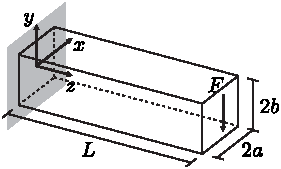
\includegraphics[width=0.5\textwidth]{bishop-beam-geometry}
% 	\caption{Cantilever beam subjected to an end shear load - geometry}
% 	\label{fig:bishop-beam-geometry}
% \end{figure}

The analytical stress state for the problem is given in \cite{bishop2014displacement} and written below:

\begin{equation} \label{eq:bishop-stress}
	\begin{aligned}
		\sigma_{xx} &= \sigma_{xy} = \sigma_{yy} = 0 \text{,}\\
		\sigma_{zz} &= \frac{F}{I} yz \text{,}\\
		\sigma_{xz} &= \frac{F}{I} \frac{2a^2}{\pi^2}\frac{\nu}{1+\nu} \sum_{n=1}^{\infty} \frac{(-1)^n}{n^2} \text{sin}\left(n\pi x/a\right) \frac{\text{sinh}\left( n\pi y/a \right)}{\text{cosh}\left( n\pi b/a \right)} \text{,}\\
		\sigma_{yz} &= \frac{F}{I} \frac{b^2-y^2}{2} + \frac{F}{I}\frac{\nu}{1+\nu} \left[ \frac{3x^2-a^2}{6} - \frac{2a^2}{\pi^2} \sum_{n=1}^{\infty} \frac{(-1)^n}{n^2} \text{cos}\left(n\pi x/a\right) \frac{\text{cosh}\left( n\pi y/a \right)}{\text{cosh}\left( n\pi b/a \right)}  \right]\text{,}\\
	\end{aligned}
\end{equation}

\noindent where $F=\int_{-b}^{b}\int_{-a}^{a}\sigma_{yz}dxdy$ and $I=4ab^3/3$ is the second moment of area about the $x$-axis. The following displacement field is obtained by integrating Equations \eqref{eq:bishop-stress} and enforcing compatibility constrains:

\begin{equation} \label{eq:bishop-displacement}
	\begin{split}
		u_x & = -\frac{F\nu}{EI} xyz \text{,}\\
		u_y & = \frac{F}{EI} \left[ \frac{\nu}{2}\left(x^2-y^2\right)z - \frac{1}{6}z^3 \right] \text{,}\\
		u_z & = \frac{F}{EI} \left[ \frac{1}{2y}\left(\nu x^2+z^2\right)z + \frac{1}{6}\nu y^3 +(1+\nu) \left(b^2 y -\frac{1}{3}y^3\right) -\frac{1}{3}a^2 \nu y \right. \\
		&\qquad\quad \left.-\frac{4a^3\nu}{\pi^3} \sum_{n=1}^{\infty} \frac{(-1)^n}{n^3} \text{cos}\left(n\pi x/a\right) \frac{\text{sinh}\left( n\pi y/a \right)}{\text{cosh}\left( n\pi b/a \right)} \right] \text{.}
	\end{split}
\end{equation}

For the analyses that follow, we kept the number of terms in the series above bounded to $n=5$. The exact solution evaluated on the boundaries of the beam is used to define the boundary conditions for the numerical analysis. At $z=0$, the exact normal and tangential displacements computed according to Eq. \eqref{eq:bishop-displacement} are prescribed, whereas surface tractions in accordance to Eq. \eqref{eq:bishop-stress} are applied on the other five faces.

Two types of partitions are used, one with hexahedral $\mathcal{S}$-elements and the other one with tetrahedral \textcolor{red}{$\mathcal{S}$}-elements. For both cases, the average element size is computed as $h_e=1/2^{n}$, where $n=\{0,1,2,3,4\}$. The coarsest ($h_e=1$) and finest ($h_e=0.0625$) meshes for each partition are shown in Figure \ref{fig:bishop-meshes}. The first analysis is carried out keeping $\nu=0.3$ as in the reference \cite{bishop2014displacement}, and a convergence test is performed for the displacement, pressure, stress and mass conservation L$^2$-norm errors, defined for the displacement as:

\begin{equation} \label{eq:bishop-errors}
	\left\| \mathbf{u} - \mathbf{u}^h \right\|_{L^2} \doteq \left[ \sum_{e=1}^{n} \int_{\Omega_e} \left(\mathbf{u} - \mathbf{u}^h\right)^2 d\Omega_e\right]^{1/2} \text{.}\\
\end{equation}

% \begin{figure}[H]
% 	\centering
% 	\subfloat[Hexahedral meshes. Coarsest (left) and finest (right)]{\includegraphics[width=1.0\textwidth]{bishop-hex-meshes}}\hfill
% 	\subfloat[Tetrahedral meshes. Coarsest (left) and finest (right)]{\includegraphics[width=1.0\textwidth]{bishop-tet-meshes}}
% 	\caption{Cantilever beam subjected to an end shear load - meshes used for the convergence test}
% 	\label{fig:bishop-meshes}
% \end{figure}

The convergence results for the aforementioned errors are shown in Figures \ref{fig:bishop-convergence-nu-03-hex}-\ref{fig:bishop-convergence-nu-03-tet}. The results show optimal convergence rates of $k+1$ for the displacement and $k$ for the remaining variables with both types of partitions. Figure \ref{fig:bishop-snapshot} plots the displacement, pressure, normal and shear stresses distributions obtained with the finest hexahedral mesh using $k=2$ over the deformed configuration of the beam. The results qualitatively agress with the reference solution, which is a strong indication of the accuracy of the proposed formulation.

% \begin{figure}
%     \centering
%     \subfloat[\label{fig:bishop-convergence-nu-03-a}Displacement]{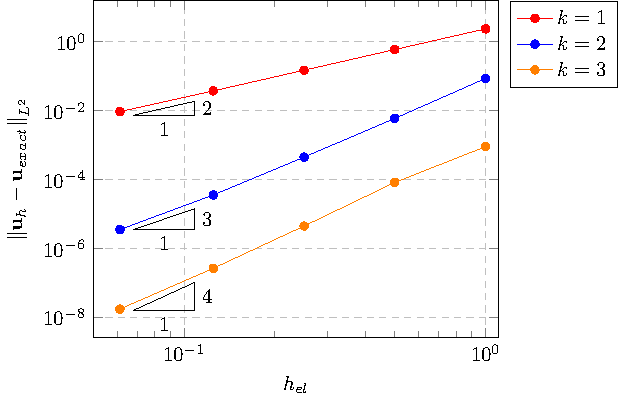
\includegraphics[trim={0cm 0cm 2.0cm 0cm},clip,scale=0.75]{Figures/bishop-disp-03.pdf}} \hfill
%     \subfloat[\label{fig:bishop-convergence-nu-03-b}Pressure]{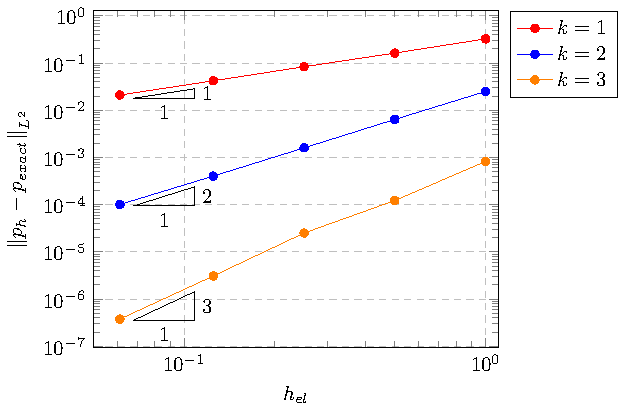
\includegraphics[trim={0cm 0cm 2.0cm 0cm},clip,scale=0.75]{Figures/bishop-pres-03.pdf}}
%     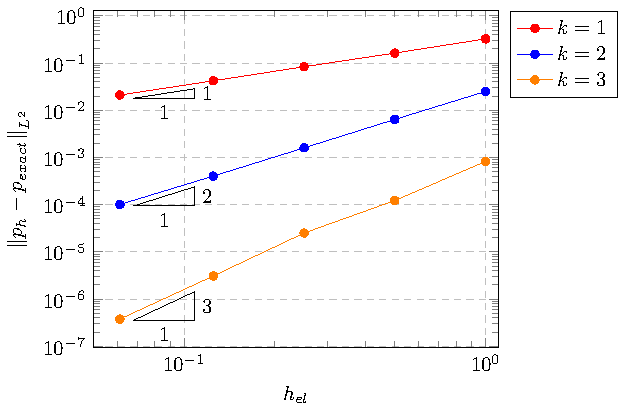
\includegraphics[trim={8.5cm 0cm 0cm 0cm},clip,scale=0.75]{Figures/bishop-pres-03.pdf}
%     \subfloat[\label{fig:bishop-convergence-nu-03-c}Stress]{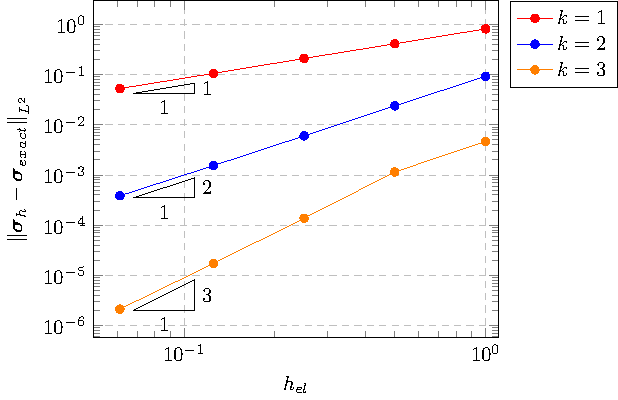
\includegraphics[trim={0cm 0cm 2.0cm 0cm},clip,scale=0.75]{Figures/bishop-stress-03.pdf}} \hfill
%     \subfloat[\label{fig:bishop-convergence-nu-03-d}Divergence]{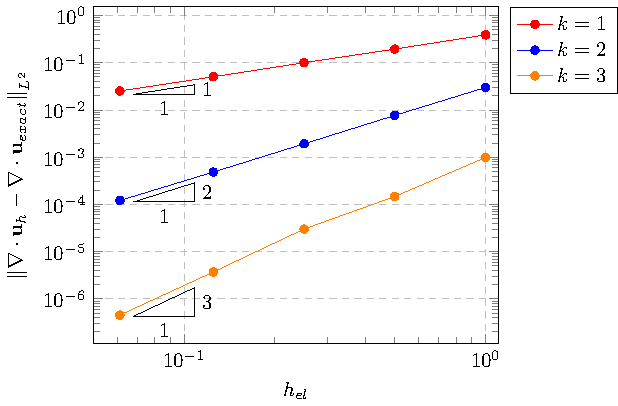
\includegraphics[trim={0cm 0cm 2.0cm 0cm},clip,scale=0.75]{Figures/bishop-div-03.pdf}}
%     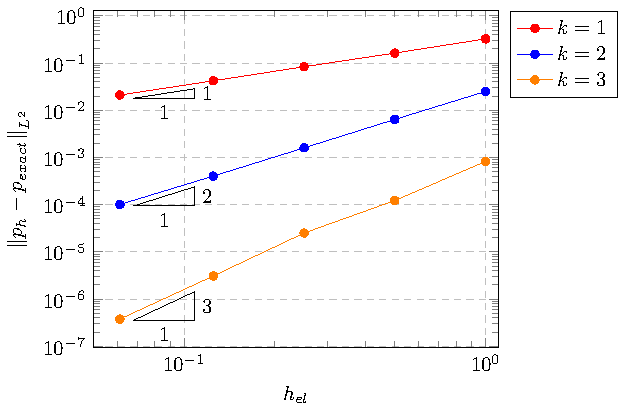
\includegraphics[trim={8.5cm 0cm 0cm 0cm},clip,scale=0.75]{Figures/bishop-pres-03.pdf}
%     \caption{Cantilever beam subjected to an end shear load - convergence analysis for the compressible case ($\nu=0.3$)}
%     \label{fig:bishop-convergence-nu-03}
% \end{figure}

% \begin{figure}
%     \centering
%     \subfloat[\label{fig:bishop-snapshot-a}Displacement]{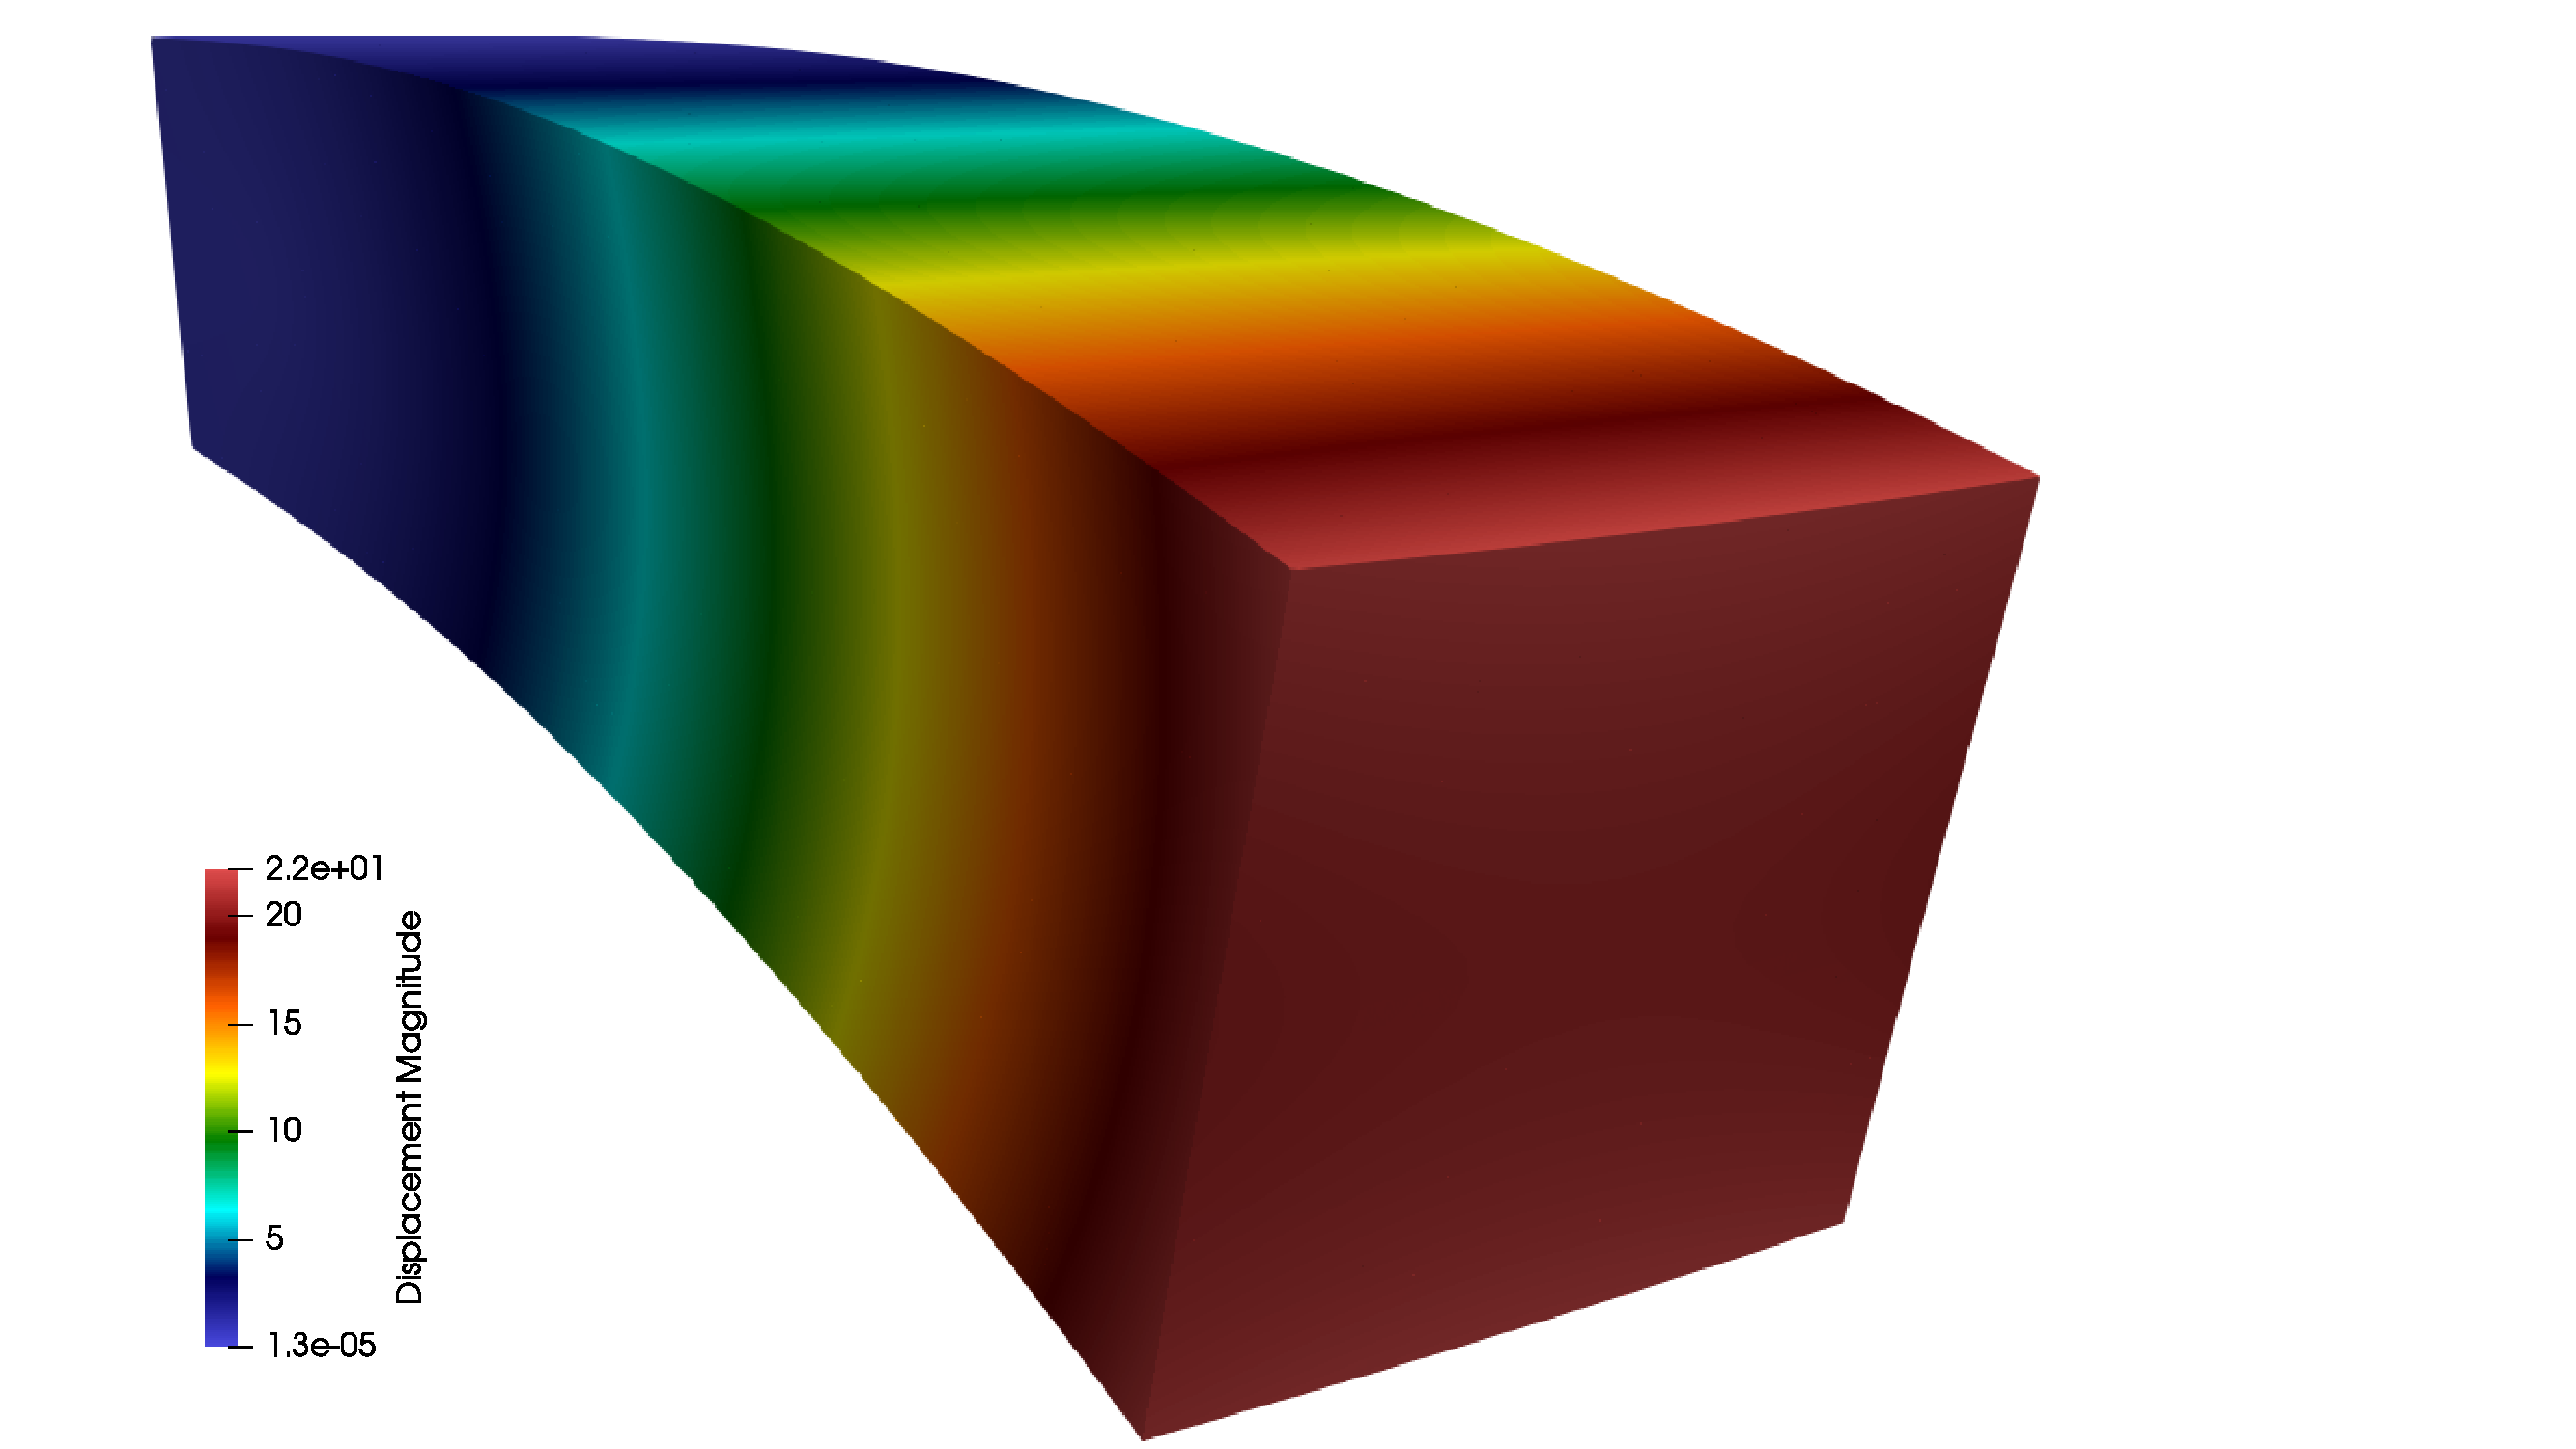
\includegraphics[trim={2.5cm 0cm 9.2cm 0cm},clip,scale=0.2]{Figures/bishop-snapshot-a.pdf}} \hfill
%     \subfloat[\label{fig:bishop-snapshot-b}Pressure]{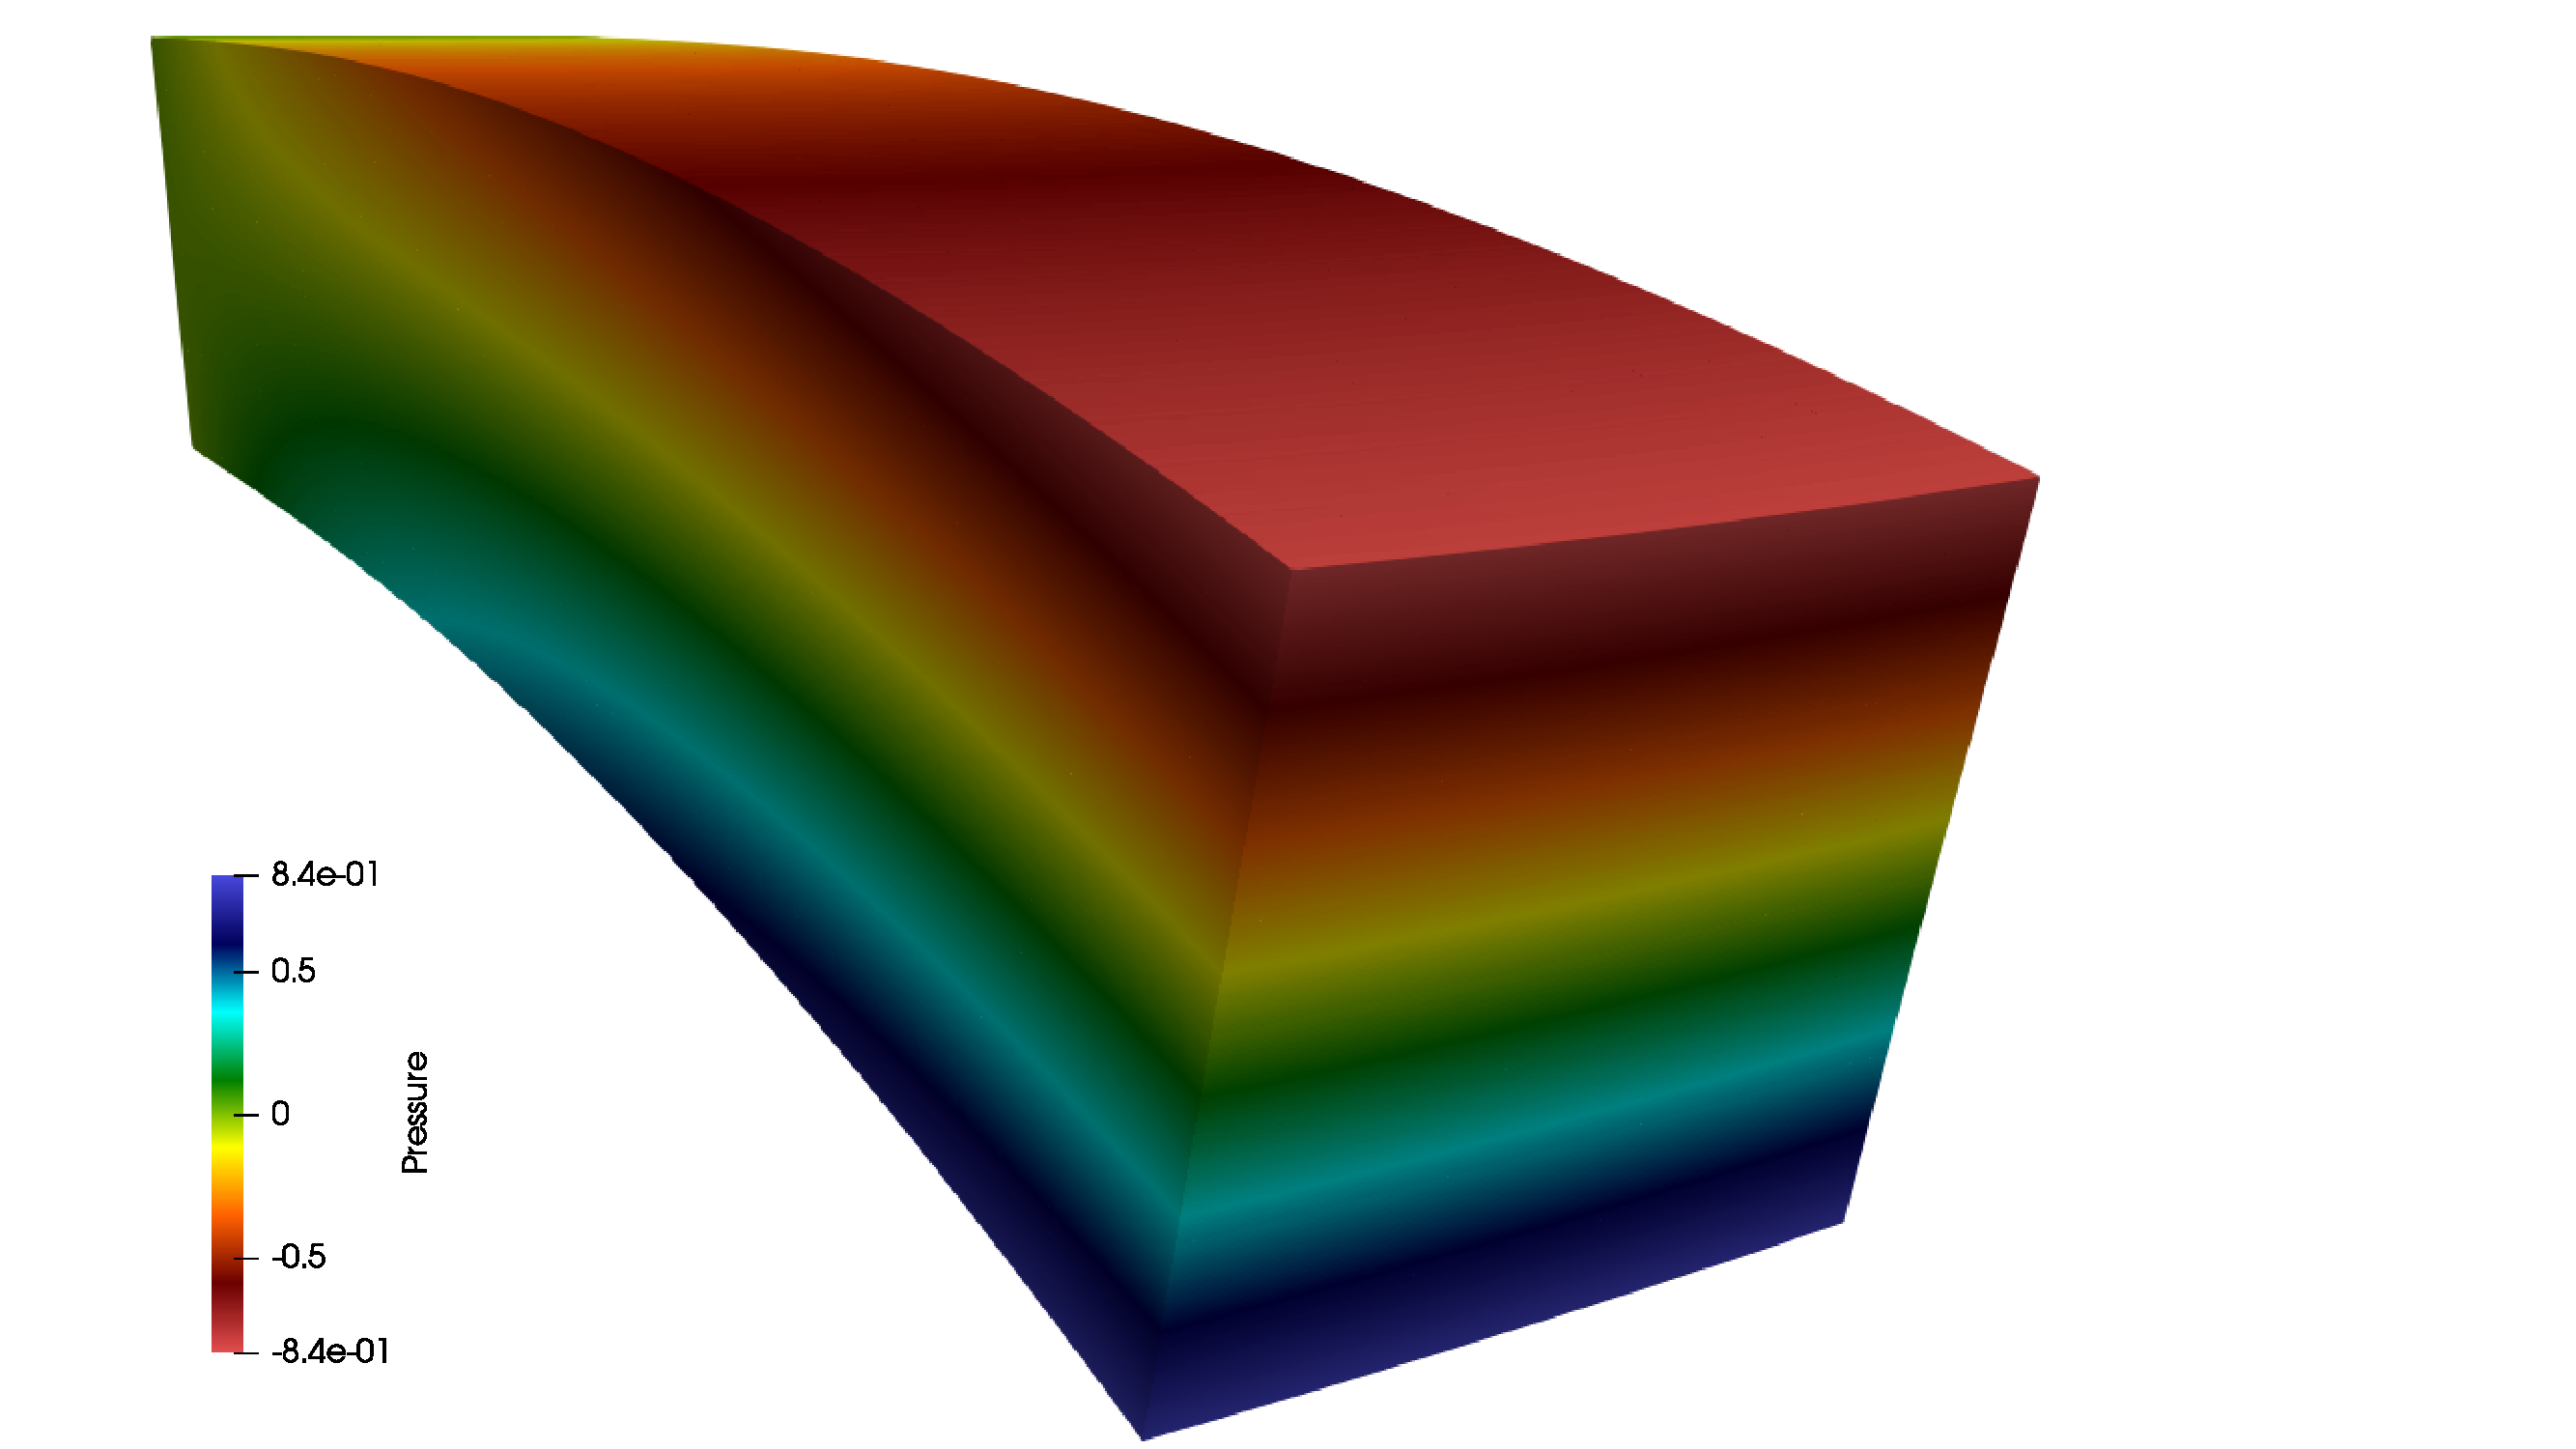
\includegraphics[trim={2.5cm 0cm 9.2cm 0cm},clip,scale=0.2]{Figures/bishop-snapshot-b.pdf}} \\
%     \subfloat[\label{fig:bishop-snapshot-c}Normal stress $\sigma_{zz}$]{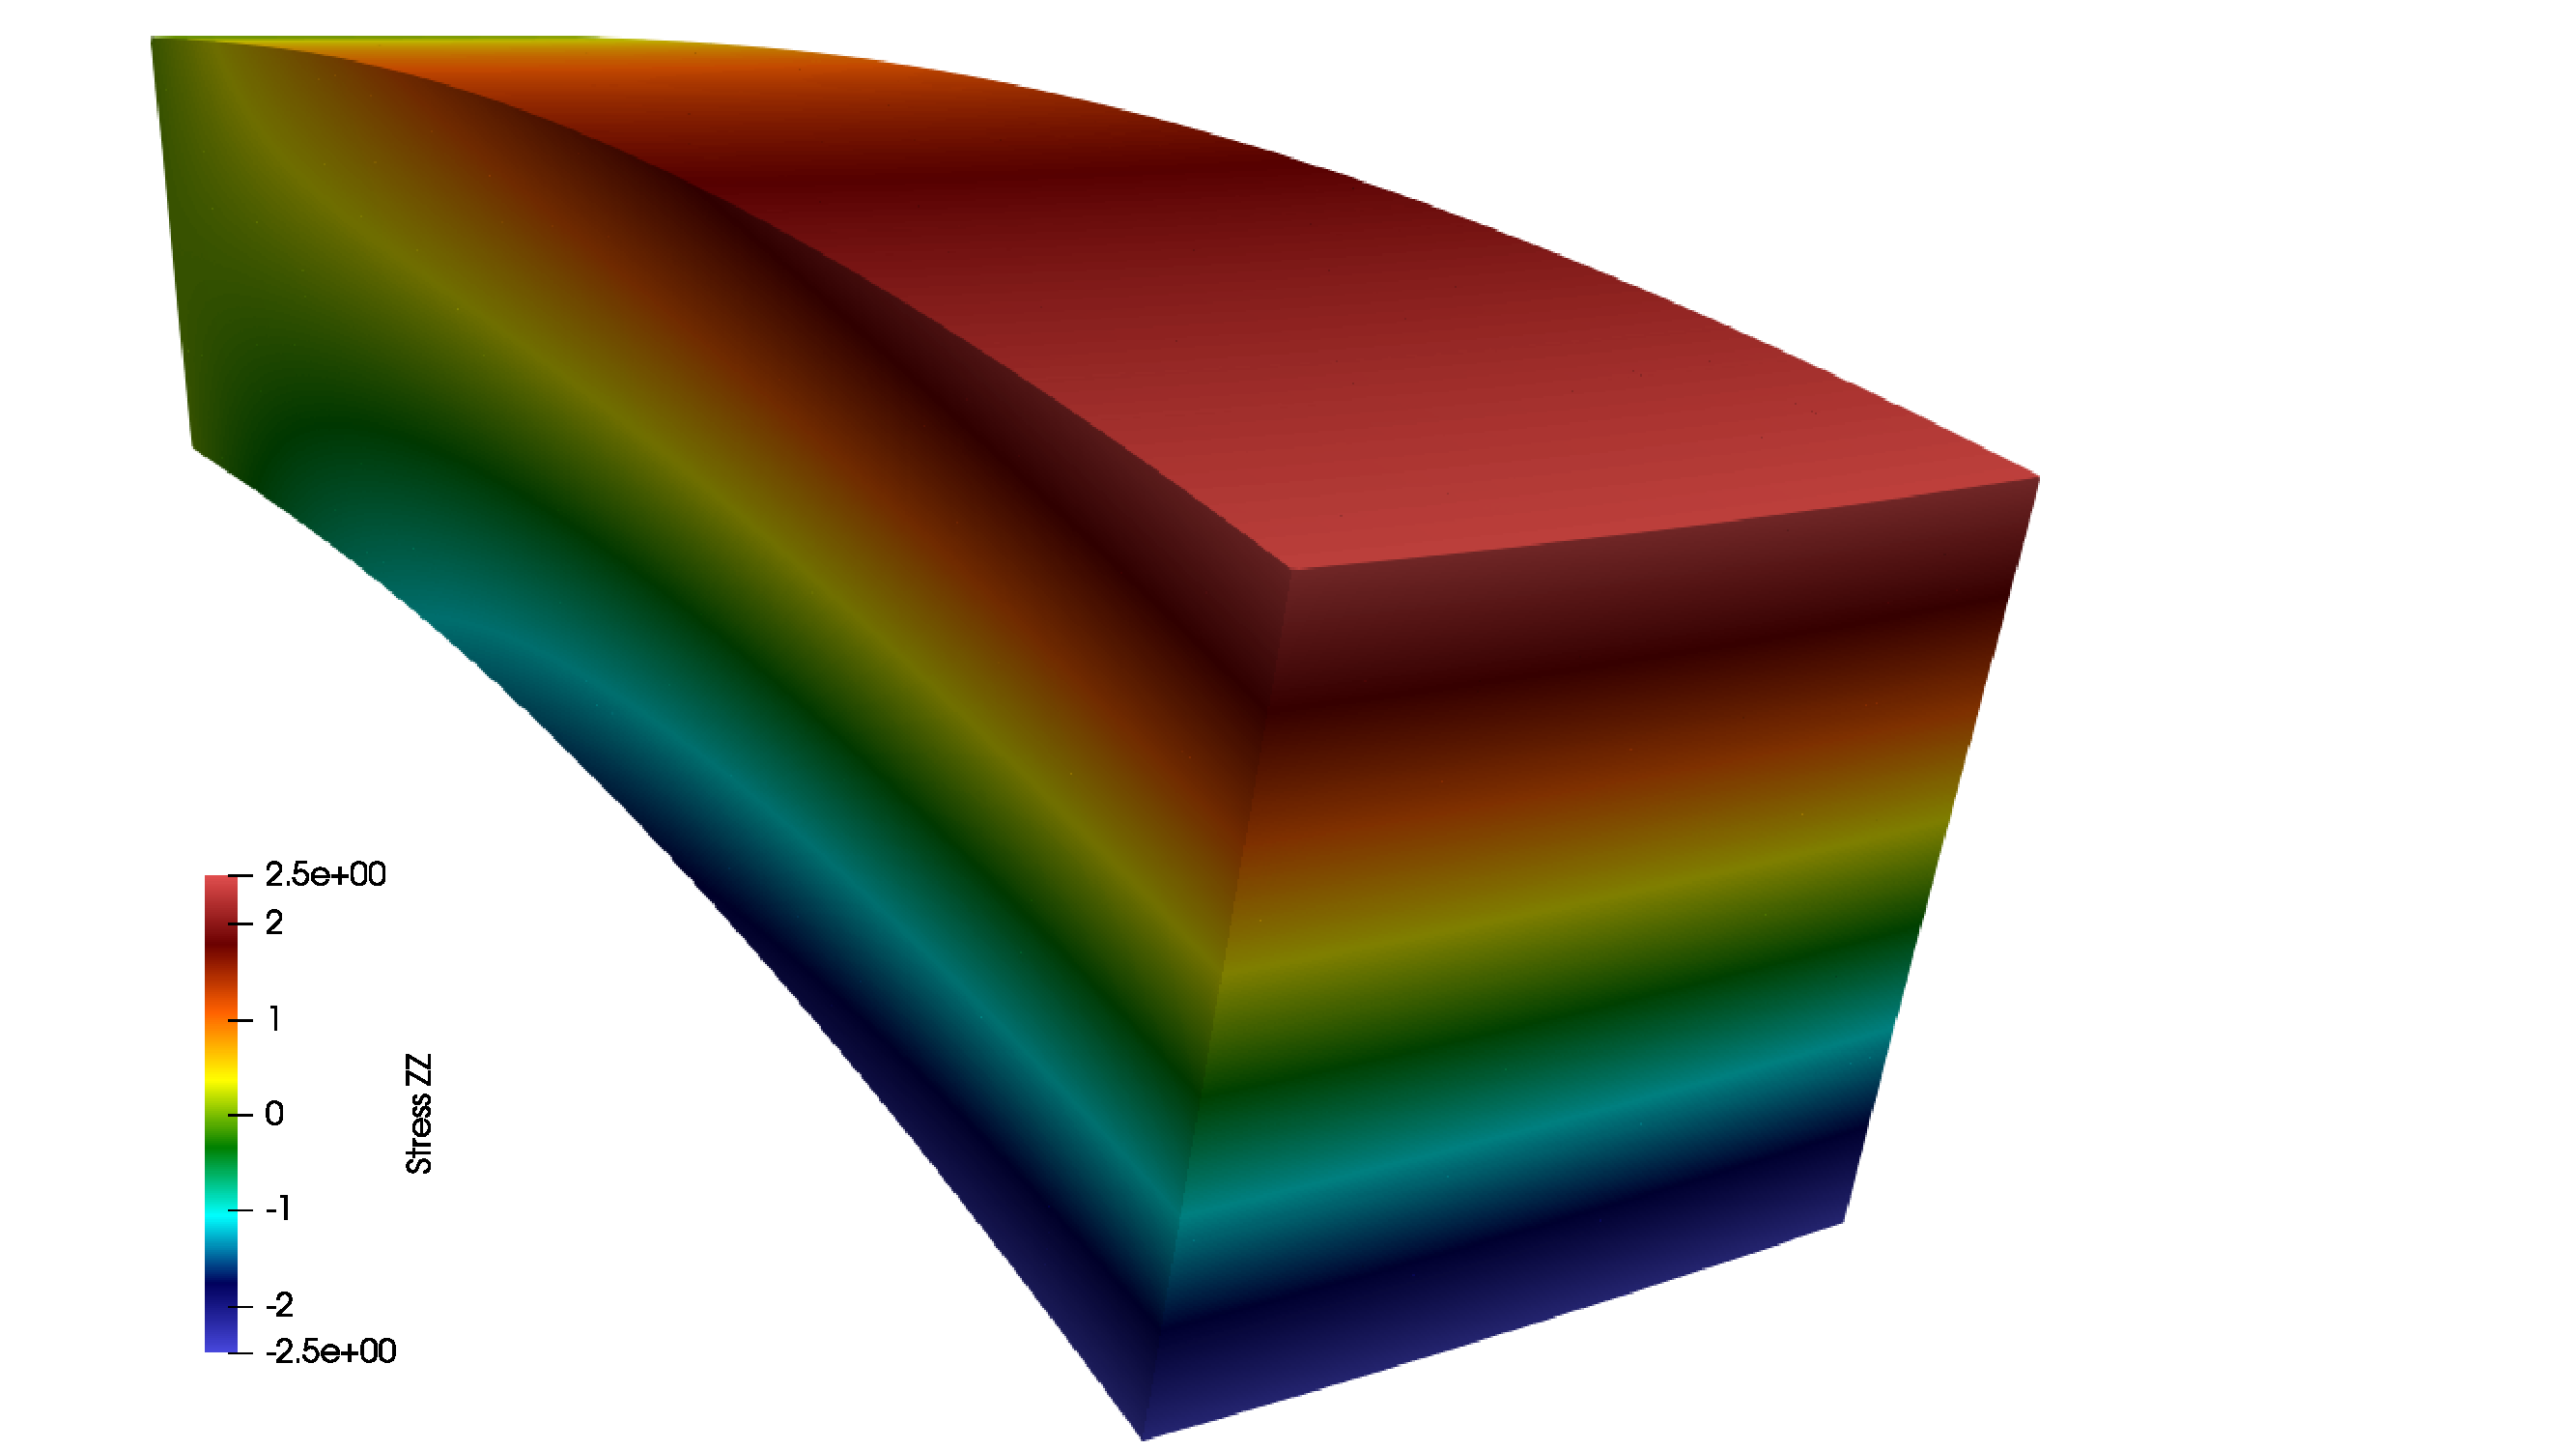
\includegraphics[trim={2.5cm 0cm 9.2cm 0cm},clip,scale=0.2]{Figures/bishop-snapshot-c.pdf}} \hfill
%     \subfloat[\label{fig:bishop-snapshot-d}Shear stress $\sigma_{yz}$]{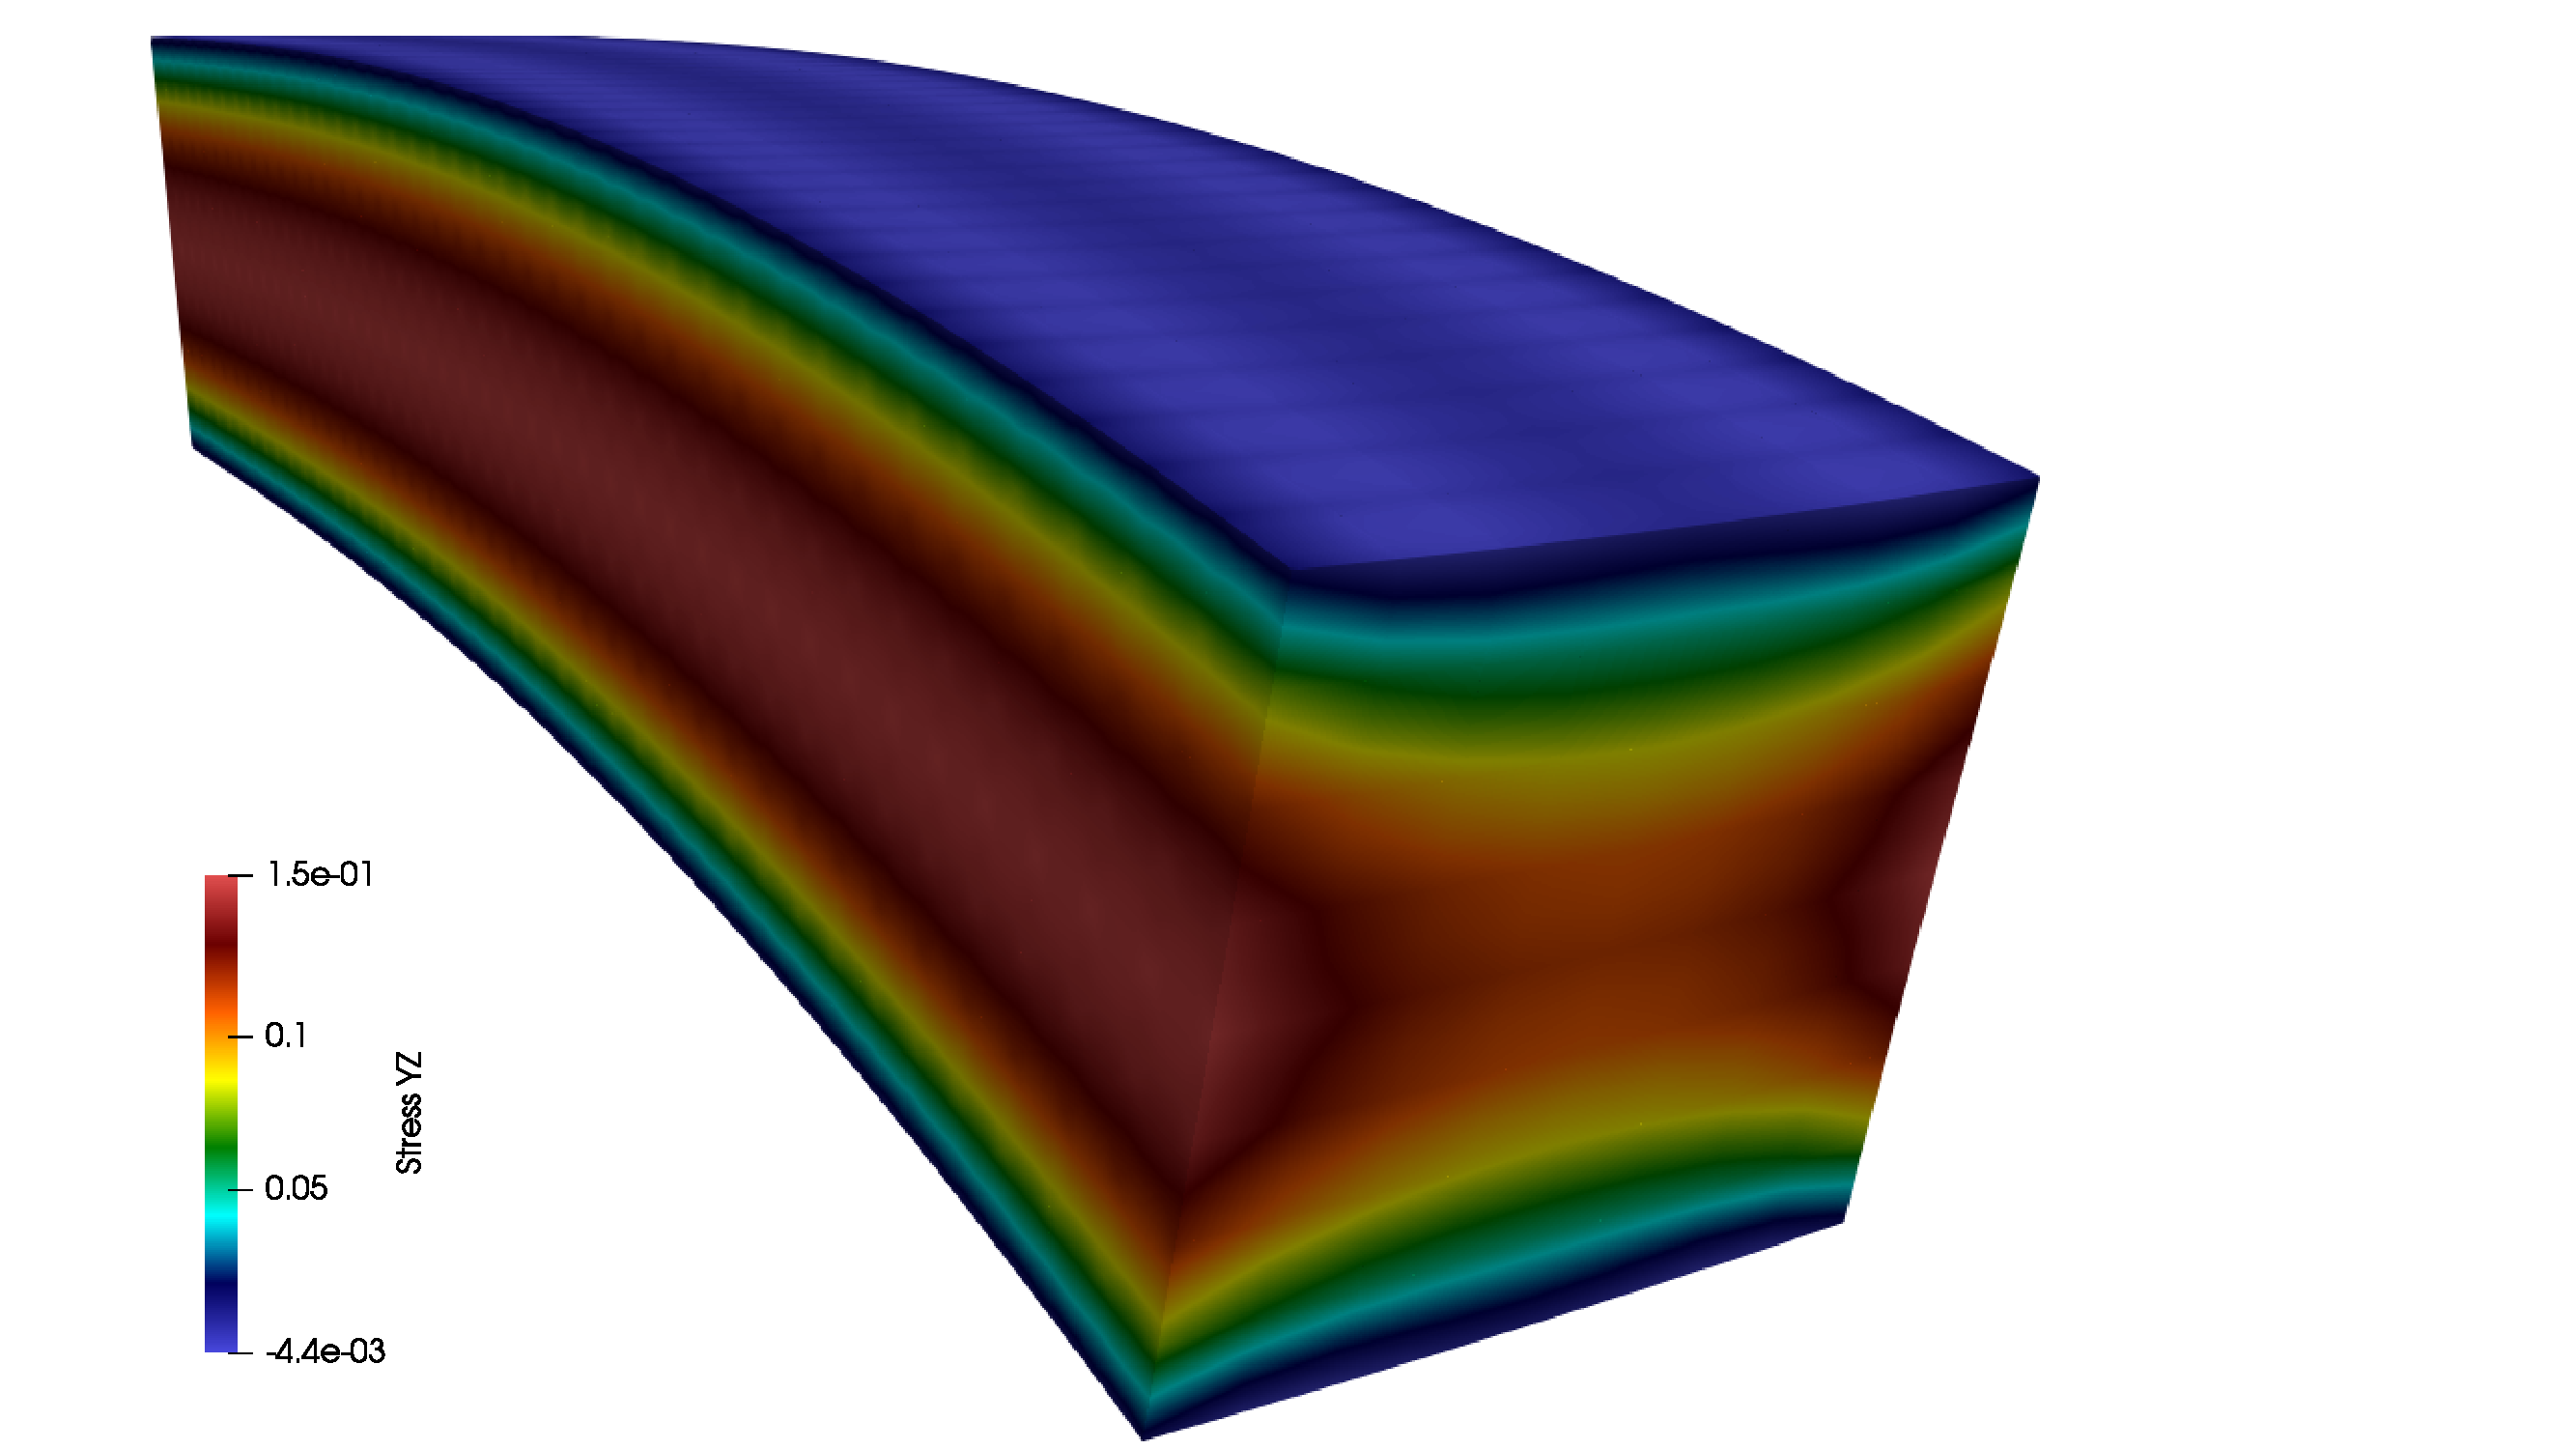
\includegraphics[trim={2.5cm 0cm 9.2cm 0cm},clip,scale=0.2]{Figures/bishop-snapshot-d.pdf}}
%     \caption{Cantilever beam subjected to an end shear load - snapshots for $\nu=0.3$}
%     \label{fig:bishop-snapshot}
% \end{figure}

In order to assess the proposed methodology in different compressibility regimes, the same analysis is performed considering $\nu=0.49$, $\nu=0.4999$, $\nu=0.499999$ and $\nu=0.5$. The convergence results are shown in Figures \ref{fig:bishop-convergence-nu-049}-\ref{fig:bishop-convergence-nu-05}, where optimal convergence rates are achieved independently of the poisson coefficient. This is a nice feature as many formulations present a locking phenomena under quasi and full incompressibility. Also, for the incompressible case ($\nu=0.5$), a divergence free displacement field is obtained even for the coarsest mesh, with the error bounded to the machine precision.

% \begin{figure}
%     \centering
%     \subfloat[\label{fig:bishop-convergence-nu-049-a}Displacement]{\includegraphics[trim={0cm 0cm 2.0cm 0cm},clip,scale=0.75]{Figures/bishop-disp-049.pdf}} \hfill
%     \subfloat[\label{fig:bishop-convergence-nu-049-b}Pressure]{\includegraphics[trim={0cm 0cm 2.0cm 0cm},clip,scale=0.75]{Figures/bishop-pres-049.pdf}}
%     \includegraphics[trim={8.5cm 0cm 0cm 0cm},clip,scale=0.75]{Figures/bishop-pres-049.pdf}
%     \subfloat[\label{fig:bishop-convergence-nu-049-c}Stress]{\includegraphics[trim={0cm 0cm 2.0cm 0cm},clip,scale=0.75]{Figures/bishop-stress-049.pdf}} \hfill
%     \subfloat[\label{fig:bishop-convergence-nu-049-d}Divergence]{\includegraphics[trim={0cm 0cm 2.0cm 0cm},clip,scale=0.75]{Figures/bishop-div-049.pdf}}
%     \includegraphics[trim={8.5cm 0cm 0cm 0cm},clip,scale=0.75]{Figures/bishop-pres-049.pdf}
%     \caption{Cantilever beam subjected to an end shear load - convergence analysis for the compressible case ($\nu=0.49$)}
%     \label{fig:bishop-convergence-nu-049}
% \end{figure}
% \begin{figure}
%     \centering
%     \subfloat[\label{fig:bishop-convergence-nu-04999-a}Displacement]{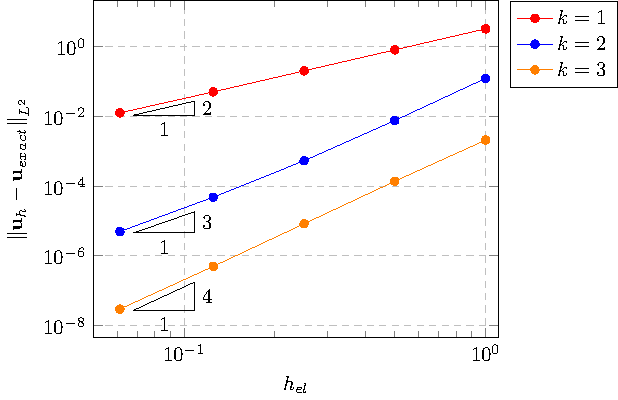
\includegraphics[trim={0cm 0cm 2.0cm 0cm},clip,scale=0.75]{Figures/bishop-disp-04999.pdf}} \hfill
%     \subfloat[\label{fig:bishop-convergence-nu-04999-b}Pressure]{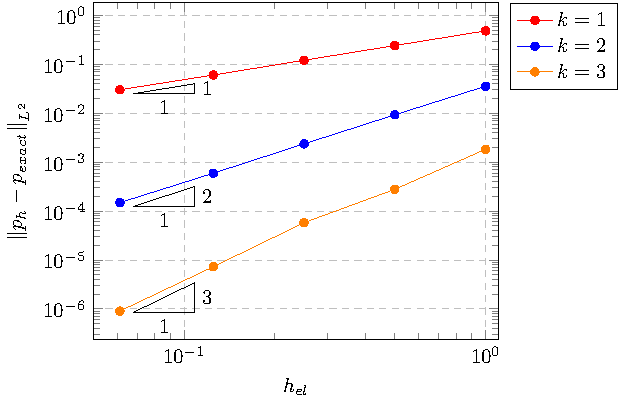
\includegraphics[trim={0cm 0cm 2.0cm 0cm},clip,scale=0.75]{Figures/bishop-pres-04999.pdf}}
%     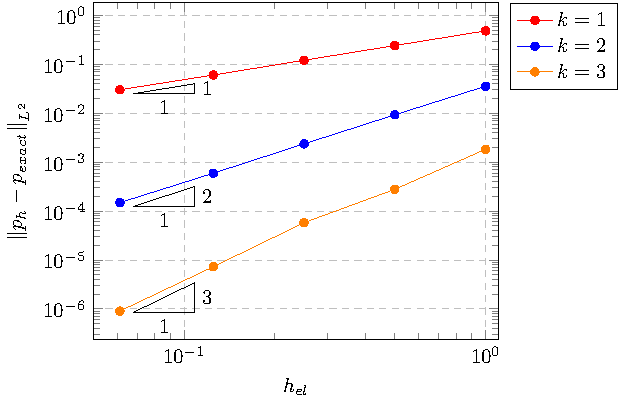
\includegraphics[trim={8.5cm 0cm 0cm 0cm},clip,scale=0.75]{Figures/bishop-pres-04999.pdf}
%     \subfloat[\label{fig:bishop-convergence-nu-04999-c}Stress]{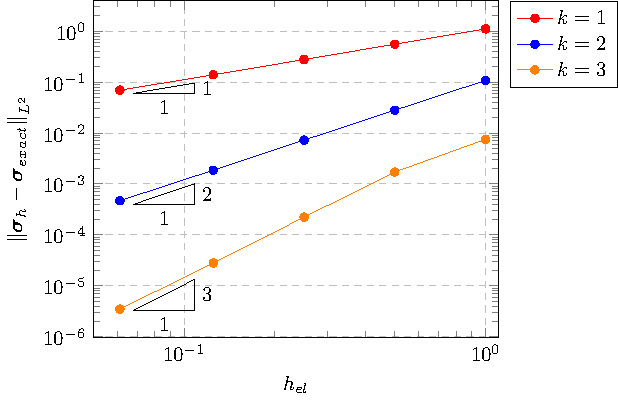
\includegraphics[trim={0cm 0cm 2.0cm 0cm},clip,scale=0.75]{Figures/bishop-stress-04999.pdf}} \hfill
%     \subfloat[\label{fig:bishop-convergence-nu-04999-d}Divergence]{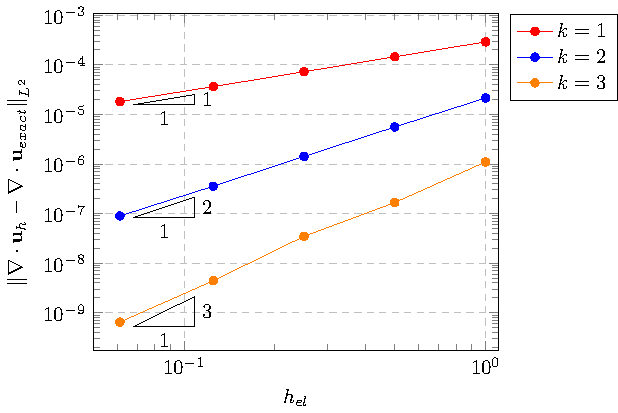
\includegraphics[trim={0cm 0cm 2.0cm 0cm},clip,scale=0.75]{Figures/bishop-div-04999.pdf}}
%     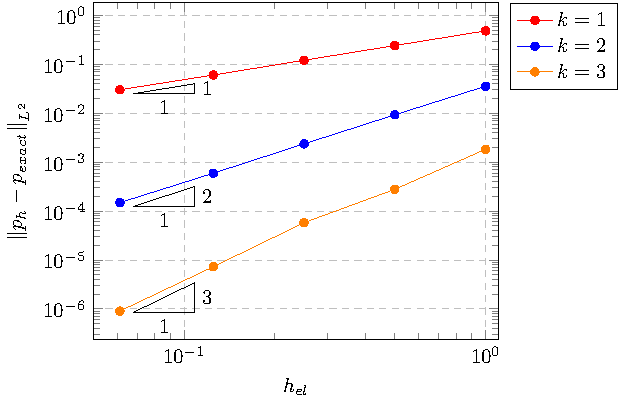
\includegraphics[trim={8.5cm 0cm 0cm 0cm},clip,scale=0.75]{Figures/bishop-pres-04999.pdf}
%     \caption{Cantilever beam subjected to an end shear load - convergence analysis for the quasi-incompressible case ($\nu=0.4999$)}
%     \label{fig:bishop-convergence-nu-04999}
% \end{figure}
% \begin{figure}
%     \centering
%     \subfloat[\label{fig:bishop-convergence-nu-0499999-a}Displacement]{\includegraphics[trim={0cm 0cm 2.0cm 0cm},clip,scale=0.75]{Figures/bishop-disp-0499999.pdf}} \hfill
%     \subfloat[\label{fig:bishop-convergence-nu-0499999-b}Pressure]{\includegraphics[trim={0cm 0cm 2.0cm 0cm},clip,scale=0.75]{Figures/bishop-pres-0499999.pdf}}
%     \includegraphics[trim={8.5cm 0cm 0cm 0cm},clip,scale=0.75]{Figures/bishop-pres-0499999.pdf}
%     \subfloat[\label{fig:bishop-convergence-nu-0499999-c}Stress]{\includegraphics[trim={0cm 0cm 2.0cm 0cm},clip,scale=0.75]{Figures/bishop-stress-0499999.pdf}} \hfill
%     \subfloat[\label{fig:bishop-convergence-nu-0499999-d}Divergence]{\includegraphics[trim={0cm 0cm 2.0cm 0cm},clip,scale=0.75]{Figures/bishop-div-0499999.pdf}}
%     \includegraphics[trim={8.5cm 0cm 0cm 0cm},clip,scale=0.75]{Figures/bishop-pres-0499999.pdf}
%     \caption{Cantilever beam subjected to an end shear load - convergence analysis for the quasi-incompressible case ($\nu=0.499999$)}
%     \label{fig:bishop-convergence-nu-0499999}
% \end{figure}
% \begin{figure}
%     \centering
%     \subfloat[\label{fig:bishop-convergence-nu-05-a}Displacement]{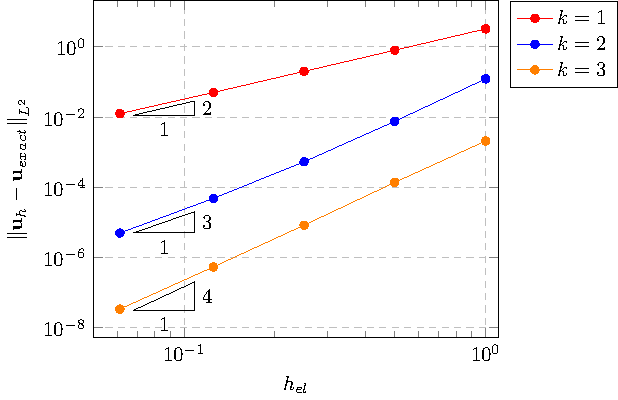
\includegraphics[trim={0cm 0cm 2.0cm 0cm},clip,scale=0.75]{Figures/bishop-disp-05.pdf}} \hfill
%     \subfloat[\label{fig:bishop-convergence-nu-05-b}Pressure]{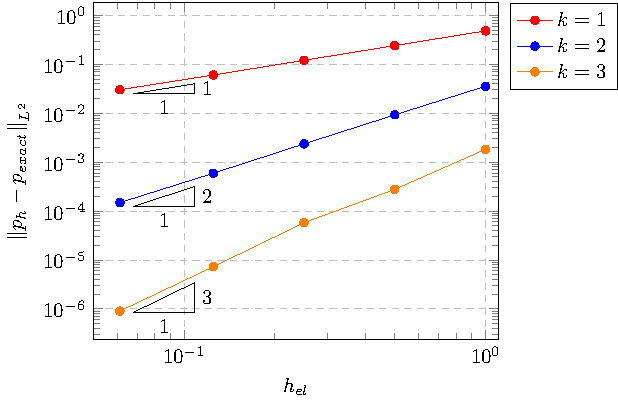
\includegraphics[trim={0cm 0cm 2.0cm 0cm},clip,scale=0.75]{Figures/bishop-pres-05.pdf}}
%     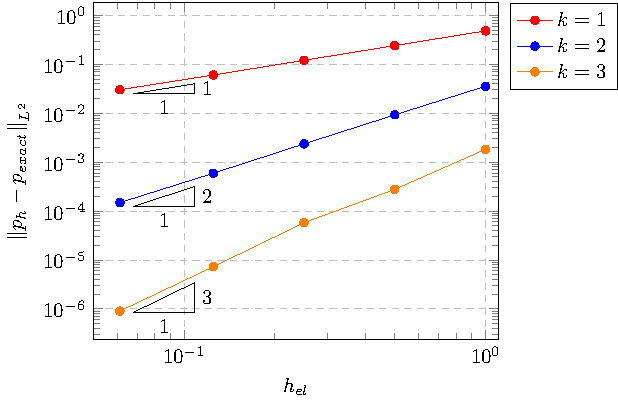
\includegraphics[trim={8.5cm 0cm 0cm 0cm},clip,scale=0.75]{Figures/bishop-pres-05.pdf}
%     \subfloat[\label{fig:bishop-convergence-nu-05-c}Stress]{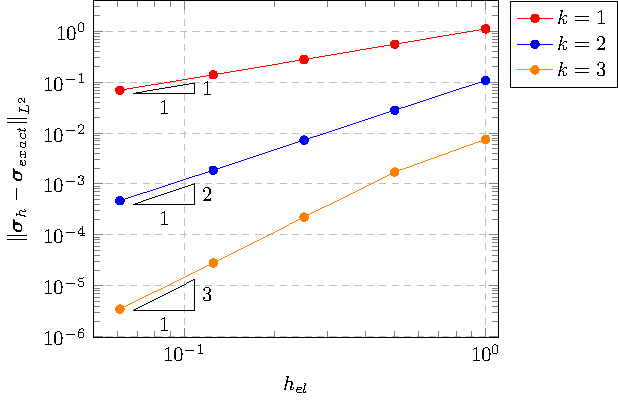
\includegraphics[trim={0cm 0cm 2.0cm 0cm},clip,scale=0.75]{Figures/bishop-stress-05.pdf}} \hfill
%     \subfloat[\label{fig:bishop-convergence-nu-05-d}Divergence]{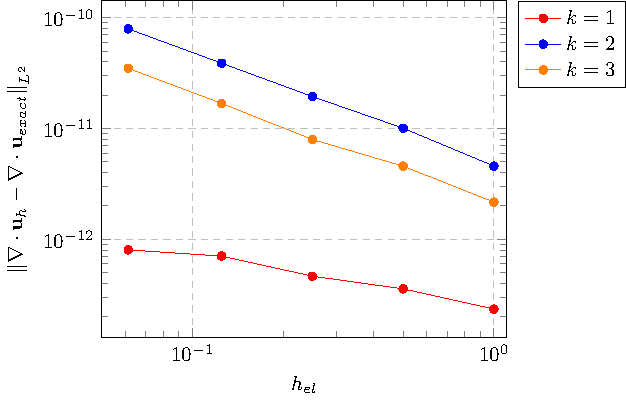
\includegraphics[trim={0cm 0cm 2.0cm 0cm},clip,scale=0.75]{Figures/bishop-div-05.pdf}}
%     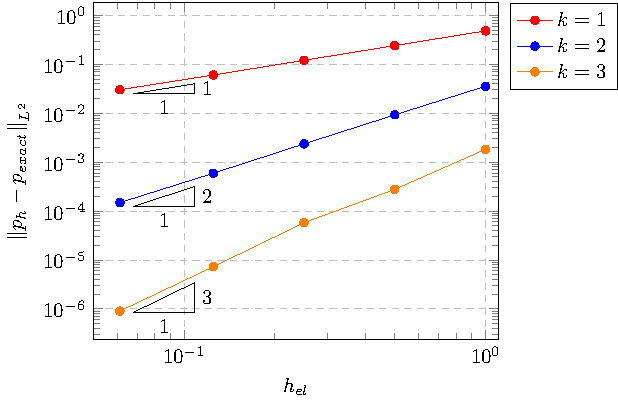
\includegraphics[trim={8.5cm 0cm 0cm 0cm},clip,scale=0.75]{Figures/bishop-pres-05.pdf}
%     \caption{Cantilever beam subjected to an end shear load - convergence analysis for the incompressible case ($\nu=0.5$)}
%     \label{fig:bishop-convergence-nu-05}
% \end{figure}

\subsection{Cook's membrane \label{subsec:cook}}

The Cook's membrane is a classical benchmark for the study of locking phenomena of incompressible or nearly-incompressible elasticity problems under shear and bending conditions. It consists of a tapered cantilever beam clamped at its left side and subjected to a shear load in the $y$ direction at the right end, according to Figure \ref{fig:cooks-geometry}. The material is assumed to have a linear behaviour as in \cite{elguedj2008b}, with a constant Young modulus $E=240.565$ MPa. Different Poisson coefficients in the range $0.3 \leq \nu \leq 0.5$ were .

% \begin{figure}[H]
% 	\centering
% 	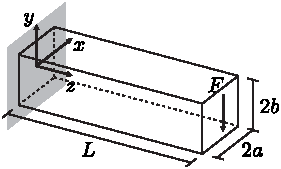
\includegraphics[width=0.5\textwidth]{bishop-beam-geometry}
% 	\caption{Cook's membrane - geometry}
% 	\label{fig:cooks-geometry}
% \end{figure}

At first, we perform a plane strain analysis using structured meshes with triangular $BDM$ and quadrilateral $\mathcal{Q}$ partitions keeping $k=1$, following by sucessive uniform refinements so that the number of elements per edge is given by $N_e=2^n$, with $n={0,1,2,3,4,5}$. The coarsest and finest meshes for both partitions are depicted in Figure \ref{fig:cooks-2d-meshes}. Figure \ref{} shows a comparison of the vertical displacement of point A for two values of $\nu$ with some numerical results available in the literature \cite{elguedj2008b,cesar1999new} and results obtained with classical $\mathcal{Q}^1$ and $\mathcal{T}^1$ quadrilateral and triangular elements, respectively, with $H^1$ functions. One notices that our approach leads to a locking-free solution and converges to the reference solutions, while the solutions obtained with classical $H^1$ shape-functions clearly exhibit an excessive bending stiffness leading to a wrong representation of the problem's cinematic.

% \begin{figure}[H]
% 	\centering
% 	\subfloat[Coarsest triangular mesh]{\includegraphics[width=0.25\textwidth]{cooks-2d-meshes-a}}
% 	\subfloat[Finest triangular mesh]{\includegraphics[width=0.25\textwidth]{cooks-2d-meshes-b}}
% 	\subfloat[Coarsest quadrilateral mesh]{\includegraphics[width=0.25\textwidth]{cooks-2d-meshes-c}}
% 	\subfloat[Finest quadrilateral mesh]{\includegraphics[width=0.25\textwidth]{cooks-2d-meshes-d}}
% 	\caption{Cook's membrane - plane strain meshes}
% 	\label{fig:cooks-2d-meshes}
% \end{figure}

A convergence test is also performed for different levels of compressibility: $\nu=0.49,$

\subsection{Application problem\label{subsec:module}}


\subsubsection{Results}


\section{Conclusions}

{\giovane A first shot, please give your contributions}
In this work a primal hybrid formulation for tridimensional elasticity problems was developed. The approximation space composed of De Rham compatible $H(\text{div})$ functions for the normal displacements and  $L^2$ functions for the pressure leads to a locally conservative scheme. A second hybridization of the tangential stresses was applied in order to obtain positive semi definite element matrices after condensing internal degrees of freedom. The property of the resulting global system is  symmetric positive-definite matrix when analysing compressible solids and a saddle point problem with a single mean pressure per element acting as a Lagrange multiplier for incompressible materials.

The formulation was tested for a cantilever beam subjected to an end shear load and the results showed optimal convergence rates of $k+1$ for the displacement and $k$ for the remaining variables independently of the poisson coefficient. The formulation was able to capture the correct stress and displacement distributions for the compressible case and a divergence free displacement field for the incompressible case. The simulation of a real scale structural hull subjected to an internal pressure qualitatively indicates that the proposed method can be applied to real engineering problems.

\bigskip\noindent {\bf Acknowledgments:} Authors  Nat, Gio, Hug, and Phil acknowledge the support from...

\appendix

\section{An Automatic Differentiation methodology to compute derivatives of H(div) shape functions \label{sec:Appendix-A.-Derivation}}

\lipsum[1-1]

\subsection*{The FAD package}

\lipsum[1-1]

%\bibliographystyle{plainnat}
\bibliographystyle{elsarticle-num} 
\addcontentsline{toc}{section}{\refname}
\bibliography{%
	references}

\end{document}
